\chapter{Caching Approaches}
\label{chapter:caching}

Since caching is an approach widely used in practice there already exists multiple caching approaches described in literature, articles on the internet and in open source code. To discover existing solutions for the problems and challenges faced in the thesis, we will research and evaluate existing caching approaches. The approaches will be analyzed and evaluated based on the criteria described in section~\ref{sec:evaluating_caching_techniques} and  requirements from section~\ref{sec:requirements}.

As already the described the most difficult part of caching is the invalidation. We will therefore start by describing existing invalidation techniques followed by how the cached values are updated and related problems. We will also describe some specific caching approaches related to web development and finish the chapter by giving an approach to picking an appropriate caching approach for a use case based on the caching criteria.

\section{Invalidation Techniques}
\label{sec:invalidation_techniques}

When the underlying data for a cached value is updated we consider the cached value as invalid. Although this sounds as a trivial part, the mechanism for invalidating the cached value can become complex depending on the requirements for the use case. To be able to navigate the existing solutions we will cover the general invalidation techniques as well as the more advanced techniques described in literature.

% section invalidation_techniques end

\subsection{Expiration-based Invalidation}
\label{subsec:expiration_based_invalidation}

In cases where it is accepted to keep the cached values stale up to a given time interval, we can use the expiration-based invalidation technique, which is the simplest invalidation mechanism since the invalidation only depends on time and not updates of underlying data. Using the expiration-based invalidation we give up consistency and the level of freshness depends on the time interval set by the programmer, but we are able to achieve immediate responses.

The expiration-based invalidation works by assigning a TTL (Time to Live) to the cached value. At some point when the TTL has expired, the cached value is invalidated. The responsibility of invalidation cached values with TTL is often placed on the cached database by piggybacking the TTL to the cached value when it is stored. This is for example supported by Redis and Memcached.

To give a sense of how the relation between when a cached value is considered valid (it is served from the cache) and when it is actually fresh, the timeline model has been applied to the expiration-based invalidation on figure~\ref{fig:timeline:expiration-based}.

\begin{figure*}[ht!]
  \centering
  \includegraphics[width=1.0\linewidth]{figures/timeline/expiration-based.pdf}
  \caption{The lifecycle of the expiration-based invalidation technique}
  \label{fig:timeline:expiration-based}
\end{figure*}

% subsection expiration_based_invalidation end

\subsection{Key-based invalidation}
\label{subsec:key_based_invalidation}

When the cached values are required to be up to date with the primary storage, we must ensure that when underlying data is updated, the depending cached values must be recomputed before the cached value can be served. The key-based invalidation gives these guarantees by giving up immediate responses since the users have to wait for computations to finish if they request an invalidated cached value. As mentioned in section~\ref{sec:evaluating_caching_techniques} the impact of this trade-off is proportional to the cache miss rate. This means that the key-based invalidation will not be suitable in cases where the computation time is too long or in cases where the cached values are updated too frequently.

Key-based invalidation works by constructing the cache key from parts of the underlying data such that the when the cached object should change, then the key also changes.~\cite{blog:key-based-invalidation}. The cached content is considered immutable and only have to be written once. This simplifies version management from the perspective of cache storage since there is no chance you read stale values if the key is assumed to be derived from the most recent version of underlying data.

The challenge of this method is to construct the key. To use this technique correctly (i.e. obtain the guarantees promised) the programmer must construct a key that is ensured to change when the cached value is considered stale. Furthermore to obtain a maximum hit rate, the key must not change when the cached value is fresh. Given that the key is optimally constructed, the timeline looks as on figure~\ref{fig:timeline:key-based}.

\begin{figure*}[ht!]
  \centering
  \includegraphics[width=1.0\linewidth]{figures/timeline/key-based.pdf}
  \caption{The lifecycle of the key-based invalidation technique}
  \label{fig:timeline:key-based}
\end{figure*}

In the web application framework, Ruby on Rails, the key construction is simplified by using a key that includes the timestamps of the last update on some underlying data. An example of this technique can be seen in code example~\ref{code:key-based-invalidation}. In this example we use the type, id and update timestamp as parts of the key. This means that the cached value is considered invalid if it is called with an entity that has a different type, id or update timestamp. The intuition behind these components is that we want a unique cache value for each entity and we want the value to be recomputed when the entity is updated.

\begin{figure}
\input{code/key_based_invalidation.py}
\caption{Example of the key-based invalidation technique}
\label{code:key-based-invalidation}
\end{figure}

The key-based invalidation performs invalidation at the moment, the cached value is requested, but it is considered invalid at the moment after the cache key components are updated (e.g. the \emph{updated\_timestamp} in the code example). This means we get interval the value is considered value and fresh are always overlapping, which means we have consistency.

A caveat of this method method is that it generates cache garbage since old versions of a cached value are not removed. To avoid the complexity of keeping track of the relations between the different, the responsibility for cleaning up is moved to the cache database. Fortunately cache databases (such as Redis and Memcached) implements different such cleanup algorithms that detects obsolete values based on some policy. One such policy called \emph{Least Recently Used (LRU)} removes the cached values that are least recently used by keeping a timestamp of when the cached values where accessed last. Another policy called \emph{Least Frequently Used (LFU)} keeps track of the frequency in which the different values are accessed and removes the ones that are least frequently accessed.

% TODO: Find litterature for these algorithms

% subsection key_based_invalidation end

\subsection{Trigger-based Invalidation}
\label{subsec:trigger_based_invalidation}

Instead of invalidating the cached value when requested, the cached values can be invalidated based on certain events triggered when the underlying data is updated. Given that invalidation triggers are located at all the places where the underlying data is updated, we can achieve the same guarantees of consistency and freshness as with key-based invalidation. The timeline model of the trigger-based invalidation on figure~\ref{fig:timeline:trigger-based} therefore looks similar to the key-based invalidation.

\begin{figure*}[ht!]
  \centering
  \includegraphics[width=1.0\linewidth]{figures/timeline/trigger-based.pdf}
  \caption{The lifecycle of the trigger-based invalidation technique}
  \label{fig:timeline:trigger-based}
\end{figure*}

Where the key is used as an invalidation mechanism in key-based invalidation, the key is static for trigger-based invalidation i.e. the key for identifying a cached value does not change in its lifetime. The actual key becomes simpler since it is only responsible for uniquely identifying the cached value, but the localization is still a challenge since the key needs to be shared between the triggers and the places where the cached value is accessed. The responsibility of invalidating the keys are then moved to the definition of event triggers.

Having a static key also has the advantage that we can locate the old/stale value after invalidation as oppose to key-based invalidation where there is no relation between the versions of cached values. Using this information we can extend the technique to be more fault-tolerant by serving a stale value in the case where a computation fails\footnote{Here we assume that the application provides more value to the client by serving a stale value compared to serving an error or nothing}. We can also extend the technique to be more flexible with relation to the properties as explained in section~\ref{subsec:trigger-based-invalidation-with-asynchronous-update} and section~\ref{subsec:write_through_invalidation}.

The simplest type of triggers are manually defined code that invalidates a given key. A code snippet for a naive implementation of manual triggers can be seen in snippet~\ref{code:manual-trigger-invalidation}. In practice the manual code triggers are often placed right after updates to the underlying data. Although this method is simple it often requires a lot of effort from the programmer and is prone to errors since it requires global reasoning of the application to identify the places where underlying data is updated.

\begin{figure}
\input{code/manual_trigger_invalidation.py}
\caption{Example of how trigger based invalidation works with manual code invalidation}
\label{code:manual-trigger-invalidation}
\end{figure}

% TODO: Consider moving the concurrency analysis to "Updating the cache" since it's related to that

Having a static key also introduces a challenge related to concurrency since we assume that there are multiple application servers. The challenge origins from the problem illustrated on figure~\ref{fig:trigger-based-concurrency-problem}, where an update to the underlying happens during the computation of a cached value. When the computation has finished it will incorrectly mark the cached value as fresh even though it is based on an old version of the underlying data, which makes it stale.

\begin{figure*}[ht!]
  \centering
  \includegraphics[width=1.0\linewidth]{figures/trigger-based-concurrency-problem.pdf}
  \caption{A scenario of the trigger-based invalidation that results in a race condition, where the cached value are being incorrectly marked as valid even though it is storing a stale value.}
  \label{fig:trigger-based-concurrency-problem}
\end{figure*}

% subsection trigger_based_invalidation end

\subsection{Trigger-based Invalidation with Asynchronous Update}
\label{subsec:trigger-based-invalidation-with-asynchronous-update}

We can extend the trigger-based invalidation by always serving the newest value from the cache and afterwards update the value asynchronously if it is stale. This way we always get an immediate response by giving up strict freshness and consistency. To give this guarantee fully the user have to wait for the computation the first time the value is requested if the application haven't `'pre-heated'` the cache i.e. included a build step before deployment that computes all cached values.

The timeline of this extension is as on figure~\ref{fig:timeline:trigger-based-with-asynchronous-update}. A naive implementation of this technique would be as the trigger-based seen in code snippet~\ref{code:manual-trigger-invalidation} with the modification that the system updates the value asynchronously instead of synchronously if no fresh value is found in the cache. The snippet for this can be found in appendix~\ref{appendix:code:trigger-based-invalidation-with-asynchronous-update}.

\begin{figure*}[ht!]
  \centering
  \includegraphics[width=1.0\linewidth]{figures/timeline/trigger-based-with-asynchronous-update.pdf}
  \caption{The lifecycle of the trigger-based invalidation technique where the value is updated in the asynchronous}
  \label{fig:timeline:trigger-based-with-asynchronous-update}
\end{figure*}

% subsection trigger-based-invalidation-with-asynchronous-update end

\subsection{Write-Through Invalidation}
\label{subsec:write_through_invalidation}

Write-through invalidation is also an extension to the trigger-based invalidation method, but instead of updating the cached values when the value is requested, the value is updated in the moment after it has been invalidated. This way we invalidate by writing through the existing version in the cache. The timeline model of this technique seen on figure~\ref{fig:timeline:write-through} is similar to the asynchronous update extension, but the time interval in which it serves a stale value is only as long as the time taken to compute the value.

\begin{figure*}[ht!]
  \centering
  \includegraphics[width=1.0\linewidth]{figures/timeline/write-through.pdf}
  \caption{The lifecycle of the write-through invalidation technique}
  \label{fig:timeline:write-through}
\end{figure*}

% subsection write_through_invalidation end

\subsection{Automatic Invalidation}
\label{subsec:automatic_invalidation}

The trigger-based invalidation is an attractive technique since it can provide guarantees with relation to freshness and consistency while allowing for flexibility by extending it. But in practice the overhead for the programmer of managing the triggers and keeping integrity becomes a burden that makes it hard to maintain. A lot of research have therefore been done in making it easier to use trigger-based invalidation.

The cached objects are based on underlying data from the primary storage system, which means that changes to the underlying data also origins from the primary store. A lot of work have been put into using the database as the source of the triggers that invalidates the cached objects.

In~\cite{paper:cache-genie} the database wrapper~\footnote{In this case in the form of an Object-Relational Mapper} is used to detect and trigger changes to the underlying data. This paper suggests a caching approach for caching database queries by declaring predefined queries with dependencies to underlying data using an extension to the database wrapper. The database wrapper is then responsible for detecting changes to underlying data and invalidate the affected cached queries. The advantage of using a database wrapper is that the caching system will still work if the database used by the wrapper is changed. On the other hand changes made to the database that are not made through the given database wrapper are not detected as a trigger, which leaves the responsibility of ensuring all changes are made through the database wrapper.

This problem can be solved using a database technology that is able to notify about changes directly from the database as done in the approach from IBM~\cite{paper:ibm, paper:ibm-extended} that uses the IBM DB2~\footnote{\url{http://www.ibm.com/analytics/us/en/technology/db2/}} database. In this approach the triggers are intercepted by a cache-manager that is able to invalidate the affected values using a dependency graph. Having a cache-manager introduces a single point of failure and potentially a bottleneck, but it allows capturing dynamic dependencies, which is required for the given application. The details about this approach will be described in section~\ref{sec:simple-object-dependence-graph}.

In~\cite{paper:liskov} a patch is made to the database such that the database is able to support so called ``invalidation streams'' that can help the caching system invalidate the affected cached values. The cache nodes stores information about how the different cache objects should be invalidated represented by invalidation tags. The invalidation stream from the storage system are then distributed across all cache nodes and used to invalidate the affected cached objects using the invalidation tags. The primary reason for these invalidation streams is to allow transactional consistency such that the primary storage and cache nodes share information that can be used to fetch a consistent set of data across both sources.

The same approach also suggests using transactions between the primary storage and the application during the computation of cached objects to capture dependencies to entities from the primary storage using the queries made in the given transaction. This way the dependencies are captured automatically, but it requires the database to implement these transactions.

\cite{paper:deploy-time} suggests using static analysis of the code to capture dependencies between the cached functions and the underlying data. In this approach the programmer must denote the data relationships, which are analyzed by the static analyzer. The static analyzer will then detect relationships between the cached functions and the underlying data as well as between different cached functions. Based on this information an object in the application process will store the dependencies for each type of dependency and not for each dependency instance. The exact dependencies are then derived using queries to the primary storage when changes are triggered. The given approach also uses a static analyzer to detect the relevant triggers.

The advantages of the deploy-time approach is that it doesn't require additional processes and it does not have to keep track of state in the form of dependencies between the different cache object instances, but these decisions have the cost that it is difficult to implement fault-tolerant measures (such as invalidation retry) as well as a poorer user experience from the performance impact of invalidation. Furthermore the approach has no mechanisms for avoiding the problem of concurrency bugs (describe in section~\ref{fig:trigger-based-concurrency-problem}).

On the other end of the granularity scale,~\cite{paper:db-driven-http} suggests a system that caches HTTP responses. It uses a sniffer process that monitors the lifetime of a HTTP request with the queries made to the storage system. Through the information captured by the sniffer, the system builds a table that maps a given HTTP resource to the queries made. The system then caches the HTTP resource that is invalidated when underlying data related to the given resource changes. This method is interesting since it allows to cache without changing the code of the web application, but it is only described at the granularity of HTTP responses since it uses the communication between the web application, storage system and cache to achieve automatic invalidation.

To be able to evaluate the techniques used in the automatic invalidation approaches described, we will divide the process into different sub problems. Automatic invalidation are based on a caching system that reacts and invalidates when changes happens to underlying data. Automatic invalidation are therefore mainly working around requests, where the client requests to update underlying data in the primary store. If we consider figure~\ref{fig:automatic-invalidation-flow} that illustrates this flow, the invalidation mechanism is responsible for step 3, 4 and 5. This involves the tasks of: \emph{triggering cache invalidation} and \emph{managing dependencies between underlying data and cached objects}. The following sections will consider these tasks and compare existing techniques.

\begin{figure*}[ht!]
  \centering
  \includegraphics[width=0.6\linewidth]{figures/automatic-invalidation-flow.pdf}
  \caption{The control flow of automatic invalidation when a client requests to update underlying data}
  \label{fig:automatic-invalidation-flow}
\end{figure*}

\subsubsection{Triggering Cache Invalidation}
\label{subsubsec:triggering-cache-invalidation}

When the client updates underlying data, the application receives a request from the client and sends a request to the primary storage to update the relevant data. To be able to react to this action, triggers have to be implemented during this flow. One technique used by~\cite{paper:cache-genie, paper:deploy-time} is to have the triggers in the application such that the application triggers invalidation when the changes from the client has been applied to the primary storage. The given techniques involves a database wrapper (in the form of an ORM) that implements callbacks invoked when it sends commands to the database. If the database wrapper is implemented using the adapter-pattern, it is possible to change the underlying database technology without changing the implementation of the caching system. This means it is easier to implement the caching system for multiple database technologies as well as change the technology for existing solutions.

Other solutions such as~\cite{paper:liskov, paper:ibm, paper:ibm-extended} assumes that the database is able to send notifications when changes are made to the database. These information from the notifications are intercepted by the caching system and converted to invalidations.~\cite{paper:liskov} uses an ``invalidation stream'' that is replicated directly across all cache nodes, which means the cache nodes has the responsibility of invalidating the correct cached objects. In~\cite{paper:ibm, paper:ibm-extended} this responsibility is extracted into a third process that converts the change notifications to invalidation of affected cache objects. A similar approach is used in~\cite{paper:db-driven-http} that uses a proxy between the application and the primary storage to ``sniff'' the database traffic and relate it to the HTTP-request of the client.

In the techniques with in-application triggers, changes to the database around the application are not captured. So if the system has the requirement that the primary storage can receive commands from multiple applications, the best solution would be to use triggers directly from the database. But this also means the system is required to use a database technology that supports this. This comparison is also shown on figure~\ref{fig:invalidation-trigger-comparison}.

\begin{figure*}[ht!]
  \centering
  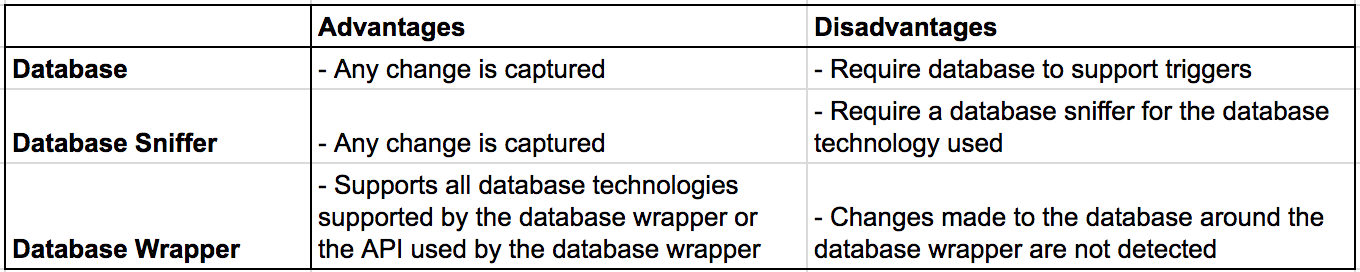
\includegraphics[width=0.9\linewidth]{figures/invalidation-trigger-comparison.png}
  \caption{Comparison of triggers for automatic invalidation}
  \label{fig:invalidation-trigger-comparison}
\end{figure*}

% subsubsection triggering-cache-invalidation end

\subsubsection{Dependency Management}
\label{subsubsec:dependency-management}

After the invalidation has been triggered, the invalidation system needs to locate the cache objects that needs to be invalidated. This involves the task of identifying and declaring dependencies such that the triggers will invalidate the affected cache objects.

Since dependency management is a burden for the programmer and affects the correctness of the cache implementation, it would be most desirable to have fully automatic dependency management, which is achieved in~\cite{paper:liskov, paper:db-driven-http}. In~\cite{paper:db-driven-http} use the technique of proxies between the different servers to sniff the traffic and thereby automatically derive dependencies between HTTP-responses and queries made during the request.~\cite{paper:liskov} runs a transaction with the database while the cached object is compute and uses information from the queries made during the transactions to derive dependencies between the underlying data and the cached object. These techniques removes the burden of cache management by having fully transparent caching, but it also means the programmer has less flexibility. Furthermore they are tightly coupled to the technologies used and makes it difficult to port the solutions to other technologies.

Other solutions relies such as~\cite{paper:cache-genie, paper:deploy-time} on the programmer declaring dependencies from the cached objects to underlying data. Since the trigger can include information about which underlying data are changed, the caching system can use the declared dependencies to invalidate the corresponding cached objects.~\cite{paper:cache-genie} supports declarations through function calls that are stored in the memory of the application. The deploy-time model suggested in~\cite{paper:deploy-time} uses static analysis of comments to allow the functions to be executed without the cache database. These techniques does not remove the burden of cache management completely, but they allow the programmer to specify the dependencies in a more declarative and robust way compared to using manual invalidation triggers.

The solution suggested by Jim Challenger et.al.~\cite{paper:ibm, paper:ibm-extended} uses dependencies declared in the content to construct an advanced dependency graph. When updates are made to content or underlying data, the affected cache objects are derived using the dependency graph. This solution is developed for a content management system, where the users can declare dependencies between the fragments of the content i.e. the dependencies are declared in each entity. This makes it unfeasible to use in application with slightly advanced data models, but it solves the problem well in the given case.

An overview of this discussion can be found in figure~\ref{fig:dependency-management-comparison}.

\begin{figure*}[ht!]
  \centering
  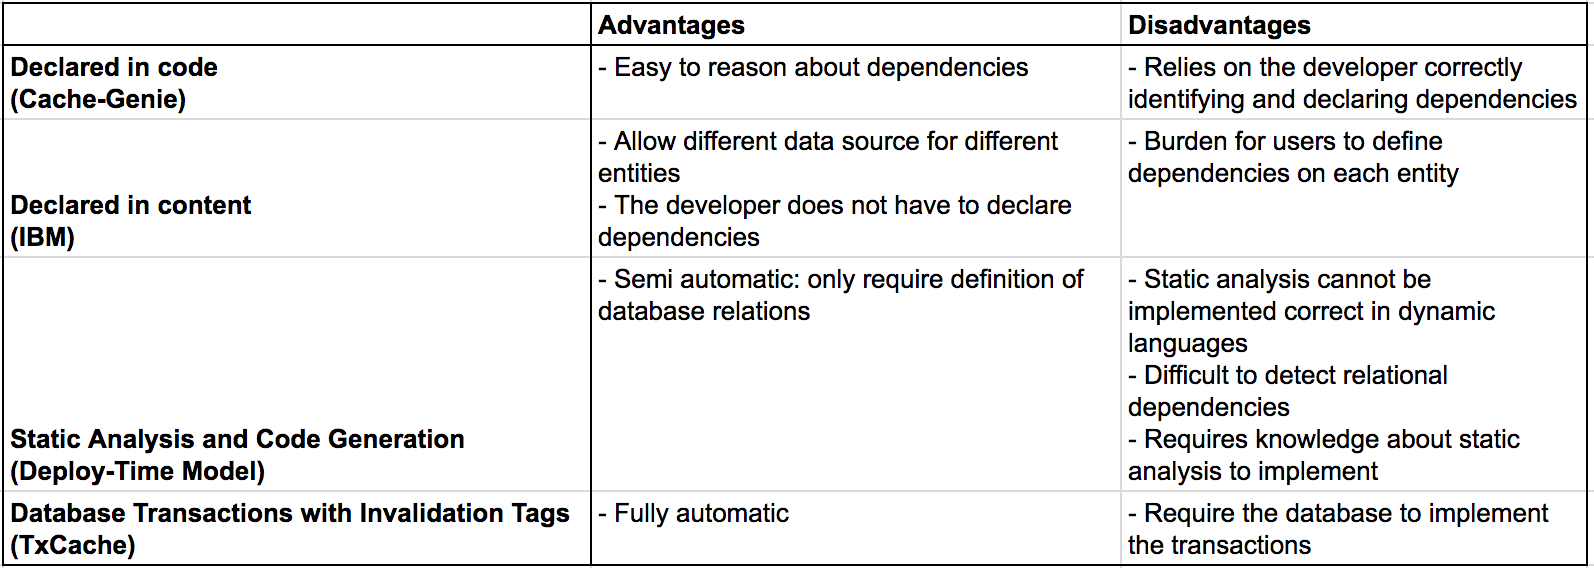
\includegraphics[width=0.9\linewidth]{figures/dependency-management-comparison.png}
  \caption{Comparison of dependency management techniques for automatic invalidation}
  \label{fig:dependency-management-comparison}
\end{figure*}

% subsubsection dependency-management end

% TODO: Mention the XML ones

% OLD WRITTEN STUFF WE'LL KEEP UNTIL THIS SECTION IS FINISHED

% TxCache suggested in~\cite{paper:liskov} uses daemon processes to monitor the database for relevant triggers. This method has the advantage that it allows multiple types of applications to manipulate the same database as opposed to~\cite{paper:cache-genie, paper:deploy-time}, where the triggers would not have been captured if the database command was made around the application. On the other hand it introduces complexity of running and monitoring the processes. With relation to database monitoring this introduces a trade-off between the complexity of the system and an assumption that multiple types of applications does not alter the same data.

% In~\cite{paper:liskov} Dan Ports et. al. uses database triggers to achieve transactional consistency for application-level caching, which ensures that any data seen within a transaction, shows a slightly stale but consistent snapshot across the storage and cache system. The database triggers are implemented using two database daemons that monitors a slightly modified version of PostgreSQL. The suggested solution, called TxCache, promises a very strong consistency guarantee, but it also comes with assumptions about the storage system and cache system used, and requires additional running daemons, which makes the full system more complex to run reliably. Furthermore these requirements contradicts flexibility and adaptability since the system assumes specific properties from the storage system and cache system, which makes it more difficult to change these components and adopt the caching system if an existing system does not use the given components.

% Another solution proposed by Chris Wasik et. al.~\cite{paper:deploy-time} uses deploy-time analysis of the code to detect dependencies between the cached functions and the dependent relations. To invalidate the cached functions automatically, the system injects code that invokes relevant invalidation callbacks in places where the underlying data is updated. Where~\cite{paper:liskov} suggests a system that comes with requirements for the architecture and technologies used, the deploy-time model is a simple system that is able to use simple key-value stores for caching and any SQL storage system. But as oppose to~\cite{paper:liskov} it does not result in as strict consistency guarantees. But despite of being a simple method, the deploy-time model is based on a system where the source code changes for different environments, which could cause errors in one environment and not in others. As an example, the code in a development or test environment could work as expected but still result in errors when deployed to a production environment, where the code is injected. Even though the deploy-time solution avoids single points of failures as with a cache manager, it needs additional operations that have to be executed in the existing procedures. In a system with complex dependencies between the procedures and underlying data, the generated source code could decrease performance that cannot be optimized by the programmer using the system.

% CacheGenie is another cache system described by Priya Gupta et. al. that uses the Object Relational Mapping (ORM) library to detect changes made to the database. Some ORM libraries already implements these triggers, which makes this approach easier to integrate into web applications that uses ORM libraries, since the caching library does not rely on database monitors. CacheGenie tries to solve the problem of managing cache invalidation when caching database queries, by letting the programmer predefine cached queries that are automatically updated in the application. CacheGenie is also based on a simple model, but each the cache definitions are based on assumptions about the specific queries and cannot be used to cache objects of a more coarse granularity.


% TODO: Make below content fit in section

% A more flexible technique is to cache functions. \cite{paper:liskov} describes a programming model for cacheable functions that essentially is functions annotated as cacheable. Although this seems attractive, it has limitations with respect to the procedures executed in the function. \cite{paper:liskov} describes the requirement of cachable functions of their programming model: “To be suitable for caching, functions must be pure, i.e. they must be deterministic, not have side effects, and depend only on their arguments and the storage layer state.” By this definition they explain that the storage layer state are treated as implicit arguments and thereby reach the classical definition of a pure function that is a transformation that always gives the same output from the same input.

% \cite{paper:deploy-time} suggests a similar programming model, where the relationships of the underlying data has to be explicitly annotated, but where the rest of the caching system is much simpler than the one described in~\cite{paper:liskov}.

% The requirement for strong consistency introduces complexity as seen with the trigger-based and key-based cache invalidation. Some objects can be cached with weak consistency, which allows much simpler caching techniques. One method is to assign a TTL (Time to Live) to the cached value. At some point when the TTL has expired, the cached object is invalidated. The invalidation can be enforced by the cache database (Redis and Memcached supports this - TODO: include references) or as part of the protocol between the client and server as with HTTP-caching explained in section~\cite{paper:web-caching-schemes}.


% subsection automatic_invalidation end

\subsection{HTTP Caching}
\label{subsec:http_caching}

% TODO: Move this to the respective caching techniques as "In HTTP-caching this is implemented using the..."

% On the other end of the granularity scale, the programmer could choose to cache the entire HTTP response send to the user. This could be the HTML documents served to the user as the website, but it could also be the JSON or XML response from an API. The HTTP protocol is the standard among web browsers to display web content and it’s widely used to communicate between web services. Since the HTTP protocol also include caching methods, which will be explained in the HTTP section, it is a very attractive caching technique among web applications.
%
% The HTTP protocol includes multiple mechanisms for controlling cache consistency that allows the web server to implement both key-based and expiration-based cache invalidation. These mechanisms are controlled using HTTP headers. The expiration-based cache invalidation information about the cache date and age is specified using the Cache-Control header. The client is then able to derive if a given resource is valid at a given time or if the resource has to be refreshed. To use key-based invalidation, the web server can attach a tag that uniquely identifies a given version of a resources (e.g. using a hash of the content). When the client sends a new request, it attaches the ETag of the last version received, and the web server can now respond with a 304 Not Modified with no content. This tells the client it can safely use the last version.
%
% Caching HTTP responses is a great technique when the same response are served to the multiple clients, but in situations where the content is updated often or personalized to each user, it becomes a less efficient technique since large documents are recomputed often. In the case where a small fragment of the content is personalized, it would be more desirable to only update that given fragment instead of recomputing the full document.
%
% The system need to cache the result of computations, which means it has to cache objects with a granularity more coarse than database queries. The HTTP protocol includes multiple features for cache management between the client and server, but it also makes the caching inflexible with relation to efficiency. In some situations HTTP responses includes shared fragments that need to be computed for each HTTP endpoint. Since the system expects long running computations, it would be more efficient to cache the result of those computations, meaning the system need to work on a granularity of fragments or functions. Since functions returns an output that could be considered a fragment, we will consider them as the same granularity.

% subsection http_caching end

% \subsection{Database Query Caching}

% TODO: Integrate stuff below in the existing chapters

% The database can be a bottleneck in the goal of achieving fast rendering of dynamic pages, because it’s often a requirement to have structured data at which you perform complex queries. In both cases the queries can become slow when the application need to scale with relation to data or users. Even though most storage systems allows indexing to optimize specific queries, it can still be difficult for the storage system to optimize in a space efficient way. One solution to this problem is to use query caches.
%
% In~\cite{paper:transparent-caching, paper:cosar} this problem is solved using a proxy caching server between the web application and the database. This allows for transparent caching that require almost no changes to the system, but unfortunately it requires a lot of work to maintain the index used for cache validation and parse the queries received from the web application. Furthermore this solution are mostly made for relational databases with SQL language and require a new implementation for it to work on different storage technologies such as document-oriented databases.
%
% \cite{paper:cache-genie} also describes a query caching solution, where the cache management is placed entirely in the application-layer. It is based on a common technology used in web application called Object Relational Mapper (ORM), where the data model is mapped to objects in the application and often the queries are made using methods on the object. Using the ORM in the Python framework Django, \cite{paper:cache-genie} implements an extension that allows common database queries to be cached and automatically updated. Compared to having a middleware caching layer, this solution has the advantage of being able to integrate with both different database technologies (within the capabilities of the ORM) and caching systems. On the other hand, it does not capture database updates made without using the ORM. This means if updates are made manually or another application uses the same database, the cached queries are not updated.

% \subsubsection{Materialized Views}
% \label{ssub:Materialized Views}
%
% Where the query caches described so far are either middle-tier or on the application-layer, caching using materialized views occurs on the database layer. Materialized views are “virtual tables” generated from other data in the database. It works by storing queries explicitly declared by the programmer. The virtual tables can be explicitly refreshed or update when the dependent data changes. Materialized views is a good solution for optimizing database queries, but since the computation occurs on the database level, the computation capabilities are limited by the database technology.
%
% Caching database queries and materialized views allows for easy and transparent caching, but it does not allow computations on the web application, which limits the applicability.

% section caching_approaches_in_web_development end

\section{Choosing the Right Caching Technique}
\label{sec:choosing_the_right_caching_technique}

% TODO: Explain/prove why this is a trade-off (ensure it is not written in caching model as well) - it probably is

% TODO: Remember both criteria and requirements

% TODO: Write a general recap/discussion on which solutions are good for what

% Write a lot about the trade-offs:

In general there is no best or correct solutions - it's a matter of choosing the solution best suited in the given context depending on the web application and specific use case. We will therefore compare the different approaches based on the parameters described in section~\ref{sec:evaluating_caching_techniques}. This comparison is illustrated on figure~\ref{fig:existing-solutions-comparison}.

\begin{figure*}[ht!]
  \centering
  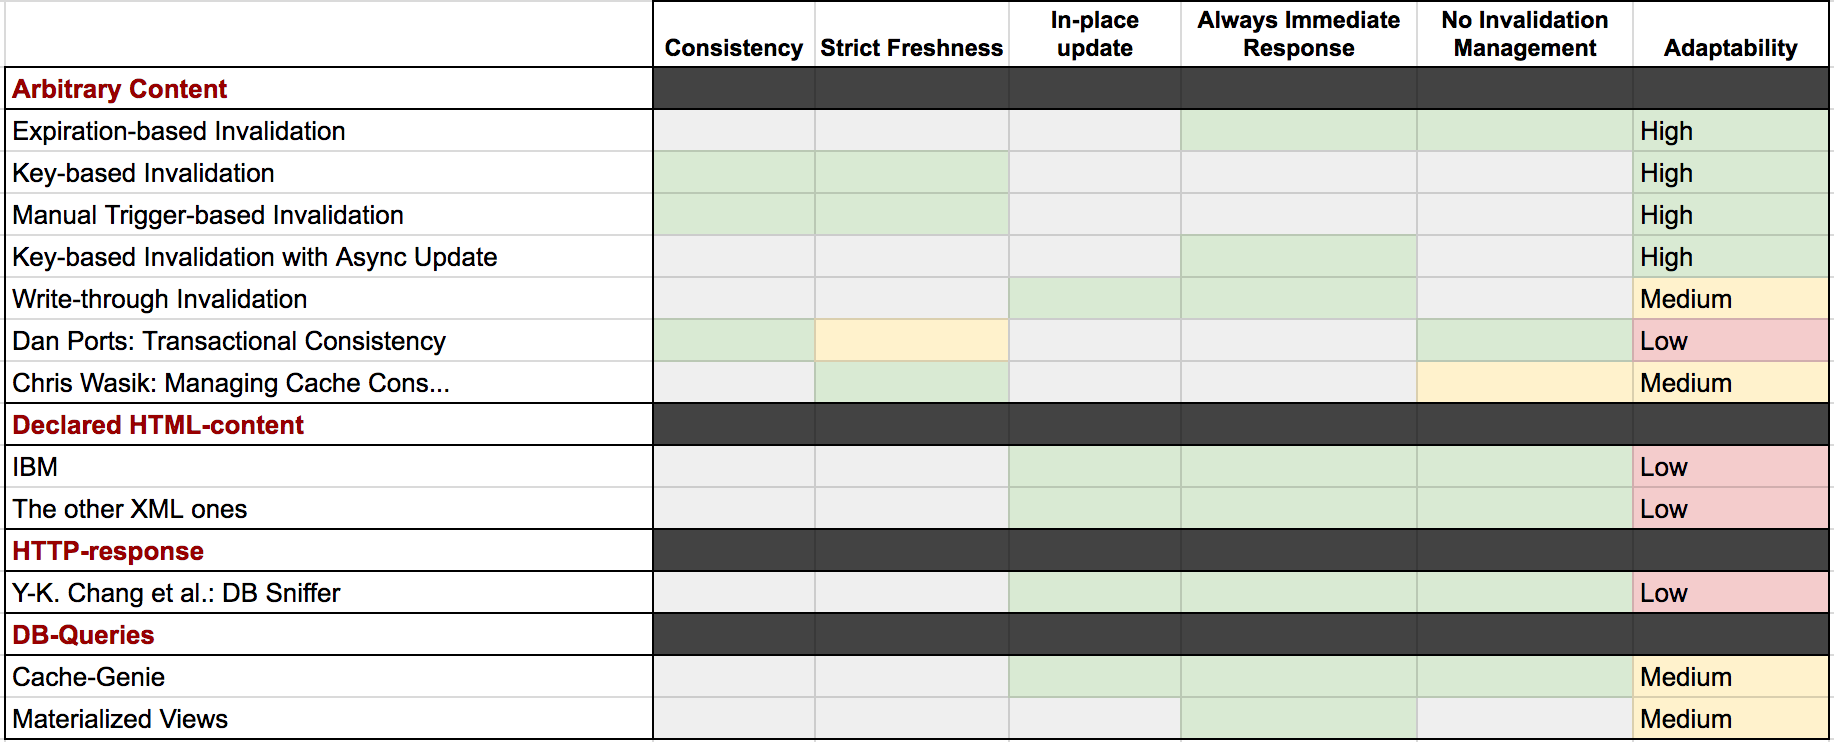
\includegraphics[width=1.0\linewidth]{figures/existing-solutions-comparison.png}
  \caption{Comparison of caching approaches}
  \label{fig:existing-solutions-comparison}
\end{figure*}

% TODO: Explain the trade-offs

From this comparison we see that some decisions have to be made between some of the parameters. At first the approach cannot both give an immediate response and provide strict freshness since if the cached computation takes $\Delta t_c$ to compute and the invalidation happens just before the request then the response time will be $~ \Delta t_c$.

% TODO: Make flow chart to decide for strategy (or maybe wait with the flow chart until after smache).

% Trade-offs:
%  - Imediate Response vs. Strict freshness

% Flexibility of solutions:
%  - Some solutions (such as Transactional Consistency) proves that their solutions
%  - can be configured on a per use-case basis.


% BELOW: Something that should be added to the sections above or the next chapter
%
% In order to keep the cached values up to date we need automatic cache invalidation. In order to achieve automatic cache invalidation with transactional consistency,~\cite{paper:liskov} describes a solution a solution that need assumptions about the storage and cache system. The system designed in this thesis does not need such strict consistency guarantees, and some of the components in the solution is therefore not necessary.
%
% The solution suggested by Jim Challenger et. al. is highly relevant to the problem of this thesis, but since the system is designed for a publishing system, it leaves some challenges that have to be solved to satisfy the requirements of this thesis.
%
% Also relevant is the paper by~\cite{paper:deploy-time} that suggests a solution that identifies dependencies and injects invalidation callbacks into the source code on deployment. This method makes the caching transparent, but it also comes with the cost that the code will be different in development and production. Furthermore the solution described does not perform write-through updates, which would also be inefficient since it would slow down existing operations that involved cache invalidations.
%
% Conclusion from this chapter: solutions exists for a lot of the sub-problems this thesis is facing, but there exists no complete solution to satisfy the requirements.

% section choosing_the_right_caching_technique end
